\chapter{Realisierung}
\section{Einführung}





\section{User Interface}
\subsection{Allgemein}
In diesem Unterabschnitt werden die Konzepte erklärt, mit welchen das User Interface realisiert wurde. Das Webinterface wurde HTML, CSS und JavaScript erstellt und als unterstützende Library wurde Twitter Bootstrap verwendet.

\subsubsection{Java Server Pages JSP}
Sämtlicher HTML Code ist in Java Server Pages (JSP) abgelegt. JSP Seiten werden auf dem Server in Java Servlets kompiliert.
\begin{figure}[H]
\centering
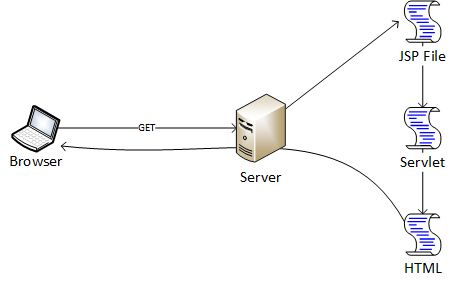
\includegraphics[scale=1]{../04_Realisierung/images/userinterface/jsp.png}
\caption{Java Server Pages}
\end{figure}
Der Client erhält über eine Web-URL vom Server generiertes HTML.

\subsubsection{Java Server Pages Standard Tag Library JSTL}
Mittels JSTL werden in dieser Applikation folgende Aufgaben erfüllt:
\begin{itemize}
\item HTML Fragmente in bestehende Container laden
\item if/else Abfragen für Darstellungen
\item Loop durch Collections im Model für die Darstellung von mehreren Objekten
\end{itemize}

In JSP Seiten wird JSTL mittels folgender Code-Zeile verwendet:
\begin{lstlisting}
<%@ taglib prefix="c" uri="http://java.sun.com/jsp/jstl/core"%>
\end{lstlisting}

Ein Loop durch eine Collection mit Hilfe von JSTP sieht folgendermassen aus:
\begin{lstlisting}
<c:forEach var="collection" items="${collection}">
</c:forEach>
\end{lstlisting}

\subsubsection{Seitenlayout}
Das Seitenlayout ist grundsätzlich sehr einfach. Die Navigation erfolgt am oberen Rand der Seite. Der gesamte Seiteninhalt befindet sich im Content-Bereich. 
\begin{figure}[H]
\centering
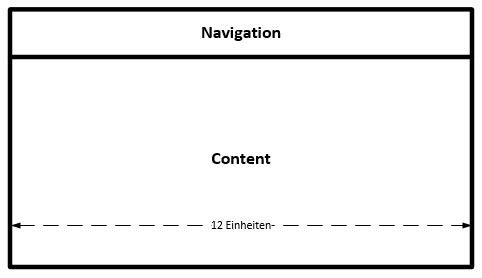
\includegraphics[scale=0.9]{../04_Realisierung/images/userinterface/seitenlayout_allgemein_large.png}
\caption{Seitenlayout Allgemein}
\end{figure}
Das Grid-System von Bootstrap teilt den sichtbaren Bereich in 12 Spalten auf. Jede Spalte besetzt immer $\frac{1}{12}$ der gesamten Fenstergrösse. Bootstrap verwendet folgende CSS Media-Queries für unterschiedliche Bildschirmtypen:
\begin{itemize}
\item Small Devices (min-width: 576px)
\item Tablets (min-width: 768px)
\item Desktops (min-width: 992px)
\item Large Desktops (min-width: 1200px)
\end{itemize}
Sämtlichen div-Containern wird angegeben, wieviele Spalten in welcher Bildschirmgrösse sie besetzen. Mit Bootstrap könnte dies folgendermassen aussehen: 
\begin{lstlisting}[language=html]
<div class="col-lg-6 col-md-6 col-sm-12 col-xs-12">
</div>
\end{lstlisting}
An diesem Beispiel besetzt dieser Div-Container auf mittelgrossen und grossen Desktops die Hälfte-, auf Tablets und Smartphones die gesamte Bildschirmbreite. Somit wird ein responsives Layout umgesetzt, dass die Applikation sowohl von mobilen-, als auch von Desktop Devices gut nutzbar ist.

\subsubsection{Navigation}
Bootstrap liefert eine ''default-navbar''. Sämtliche Navigationslinks (Home, Device, Discovery, Configurations, User Panel) befinden sich in der Navigationsleiste. Die Navigationsleiste besetzt in jeder Bildschirmgrösse die gesamte Breite.
\begin{lstlisting}[language=html]
<div class="col-lg-12 col-md-12 col-sm-12 col-xs-12">
</div>
\end{lstlisting}
\begin{figure}[H]
\centering
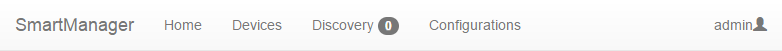
\includegraphics[scale=0.8]{../04_Realisierung/images/userinterface/navbar_lg.png}
\caption{Navigationsleiste gross}
\end{figure}

Da diese Navigationsleiste auf Smartphones schwierig zu bedienen ist, wird auf der kleinsten Bildschirmgrösse anstatt der normalen Links in der Navigation ein Hamburger-Button verwendet. Anfangs war dieser Button stark umstritten, mittlerweile wird er häufig eingesetzt, weshalb jedem Benutzer klar sein sollte, dass sich dahinter weitere Elemente befinden.
\begin{figure}[H]
\centering
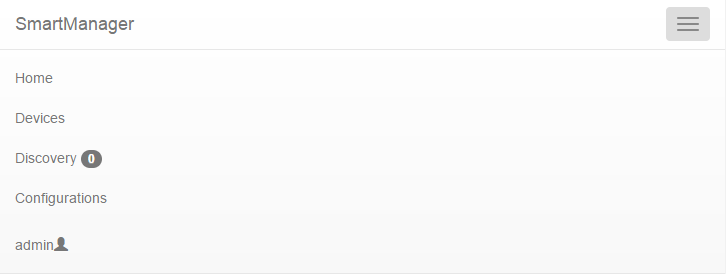
\includegraphics[scale=0.87]{../04_Realisierung/images/userinterface/navbar_xs.png}
\caption{Navigationsleiste xs}
\end{figure}

Die Navigationsleisten sind auf jeder Seite am oberen Bildschirmrand fixiert, sodass bei allfälligem Scrollen die Navigation trotzdem sichtbar bleibt.

Damit duplizierter Code auf jeder Seite verhindert wird, wird der gesamte HTML Code für die Navigation in ein eigenes JSP File ''menuFragment.jsp'' ausgelagert. Der Inhalt des JSP Files wird mittels 
\begin{lstlisting}[language=html]
<jsp:include page="../../views/menuFragment.jsp" />
\end{lstlisting}
serverseitig ins HTML gerendert.
\subsubsection{Content}
Der gesamte Content Bereich ist auf jeder Seite unterschiedlich gestaltet. Die gesamte Breite von 12 Spalteneinheiten kann verwendet werden.

\subsubsection{Asynchronous JavaScript and XML AJAX}
Damit bei der Kommunikation mit dem Server das User Interface nicht blockiert wird, werden bei sämtlichen Server-Calls AJAX verwendet. AJAX versendet Nachrichten vom Client an den Servern asynchron. Im ''success'' Attribut kann eine Callback-Funktion hinterlegt werden, welche bei erfolgreicher Antwort ausgeführt wird.

In dieser Applikation werden AJAX-Calls nach folgendem Schema ausgeführt:
\begin{lstlisting}
$.ajax({
	type : "GET/POST/DELETE",
	url : ctx + "/resource/method",
	success : function() {
		/*some callback code...*/
	},
	error : function(xhr, ajaxOptions, thrownError) {
		window.location.href = ctx + "/";
		alert(thrownError);
	}
});
\end{lstlisting}

Falls der Server mit einem Fehler antwortet, wird die Callback-Funktion im ''error''-Attribut ausgeführt. Der Benutzer wird dabei auf die Haupt-Seite umgeleitet und erhält eine Error-Meldung angezeigt.

\subsubsection{Bootbox}
An verschiedenen Stellen auf der Seite werden Pop-ups benötigt. In diesem Projekt wird die JavaScript Library ''Bootbox'' von Bootboxjs.com verwendet.

\begin{figure}[H]
\centering
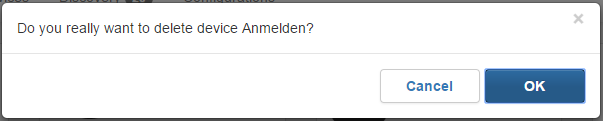
\includegraphics[scale=0.9]{../04_Realisierung/images/userinterface/bootbox.png}
\caption{Bootbox}
\end{figure}

Der JavaScript Code für die Erstellung und Verwendung der Bootbox ist leicht verständlich.

\begin{lstlisting}
bootbox.confirm({
	size : "large",
	title : "some title",
	message : content,
	callback : function(ok) {
		if (ok) {
			/*save, redirect etc.*/		
		}
	}
});
\end{lstlisting} 

Als ''message''-Attribut kann ein String oder auch HTML Code eingefügt werden.  Beim ''Callback''-Attribut kann eine Callback-Funktion hinterlegt werden. Diese wird ausgeführt, wenn das Pop-up Fenster geschlossen wird. Die if-Abfrage stellt sicher, dass der darinliegende Code nur ausgeführt wird, wenn ''OK'' auf geklickt wird.

\subsubsection{Google Maps API}
An verschiedenen Stellen auf der Seite werden Devices auf Google Maps Karten angezeigt. Dies gibt dem Benutzer eine schnelle Übersicht der Lokalitäten der IoT Devices.

Über die JavaScript-Funktion ''initMap()'' wird die (leere) Map geladen. Danach werden über die Funktion ''getLocations()'' die Locations der benötigten IoT Devices vom Server abgefragt. Über die ''insertLocations()''-Funktion werden die Punkte auf der Map eingezeichnet.

\subsection{Home}
Die Home-Seite dient als Einstiegspunkt und Übersichtsseite. Dem Benutzer sollen Informationen über die Applikation und die verwaltete Infrastruktur angezeigt werden.

\begin{figure}[H]
\centering
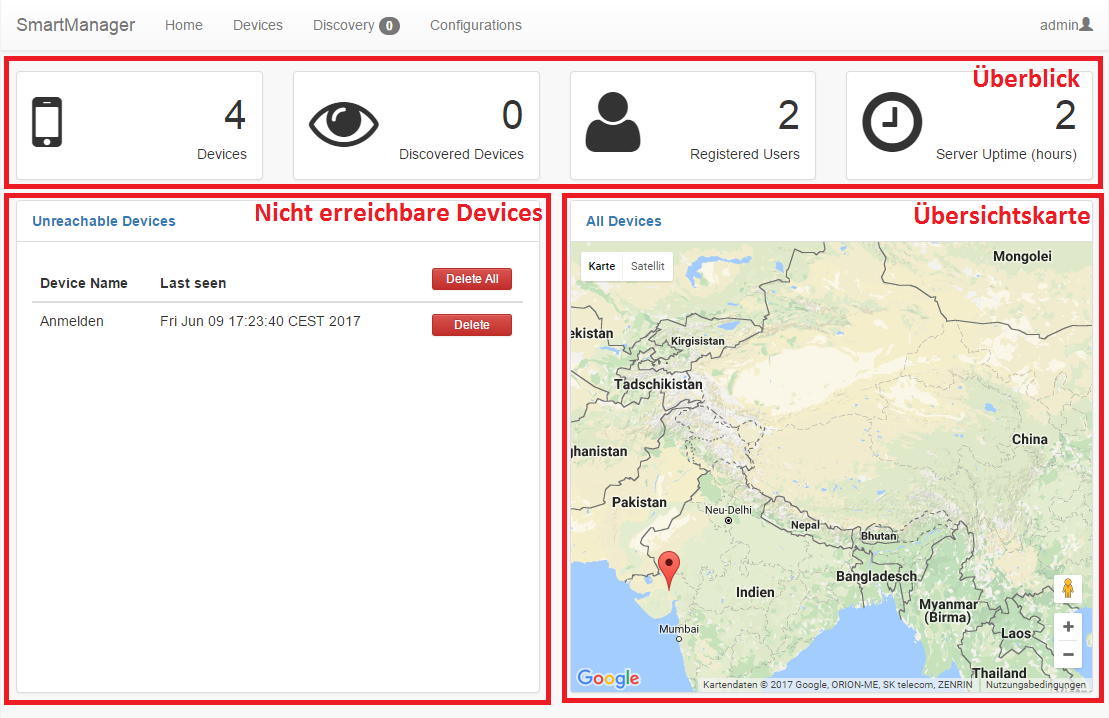
\includegraphics[scale=0.57]{../04_Realisierung/images/userinterface/home.png}
\caption{Dashboard}
\end{figure}

\subsubsection{Überblick}
In diesem Bereich werden dem Benutzer folgende vier Informationen auf den ersten Blick angezeigt:
\begin{itemize}
\item Gesamtanzahl erfasster Devices im System
\item Anzahl Devices im Discovery (noch nicht verwaltet)
\item Anzahl registrierter Benutzer
\item Server Uptime in Stunden
\end{itemize}

\subsubsection{Nicht erreichbare Devices}
Sind Devices nicht mehr erreichbar, muss dies dem Benutzer mitgeteilt werden. Hat sich ein Device mehr als 30 Minuten nicht mehr beim Server gemeldet, so erscheint es in dieser Tabelle. Klickt der Benutzer auf ''Delete'' respektive ''Delete All'', so werden die JavaScript Funktionen ''deleteUnreachableDevice(id, name)'' und ''deleteAllUnreachableDevices()'' ausgeführt. Über eine AJAX-Anfrage werden die entsprechenden Serverpfade aufgerufen.

\subsubsection{Übersichtskarte}
Auf dieser Übersichtskarte werden alle im Device gespeicherten Locations von IoT Devices angezeigt.

\newpage
\subsection{Discovery}
Auf der Discovery Seite sieht der Benutzer alle registrierten Devices. Sämtliche Devices registrieren sich am LwM2M Server. Sind sie vom Benutzer noch nicht hinzugefügt worden, so erscheinen sie auf dieser Seite.

\begin{figure}[H]
\centering
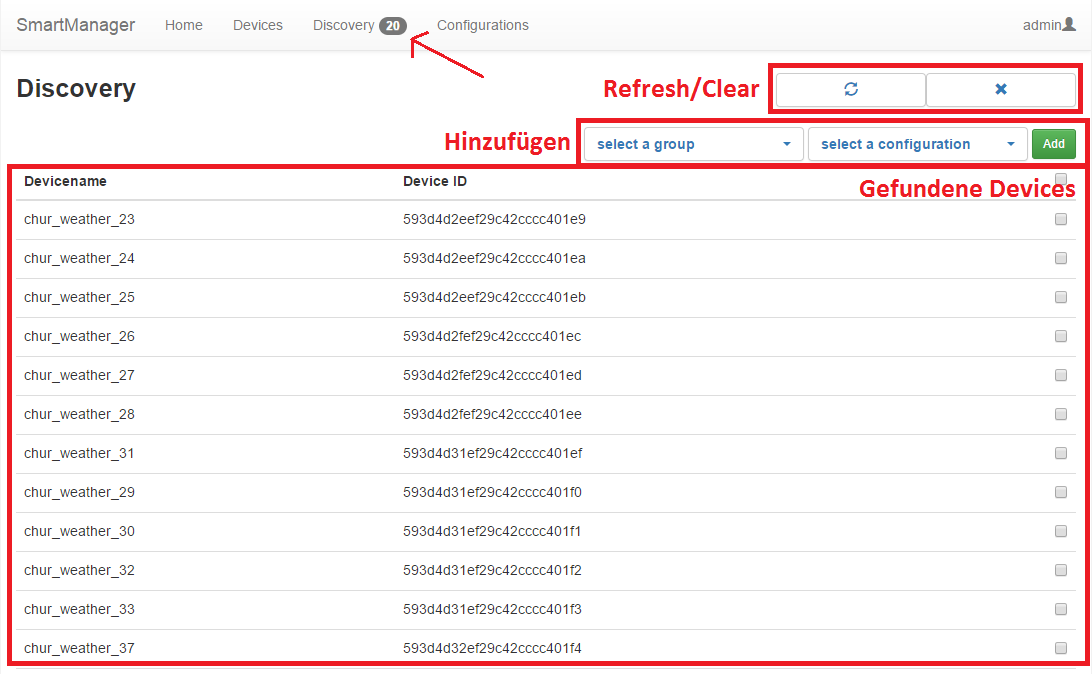
\includegraphics[scale=0.57]{../04_Realisierung/images/userinterface/discovery.png}
\caption{Discovery}
\end{figure}

\subsubsection{Gefundene Devices}
Ist ein Device vom Benutzer noch nicht hinzugefügt worden, besitzt das Attribut ''added'' den Wert ''false''. Nachdem der Benutzer das Device hinzugefügt hat, wird dem Device das Attribut ''added'' auf ''true'' gesetzt und erscheint deshalb nicht mehr.

\subsubsection{Hinzufügen}
Beim ''Add''-Button werden die selektierten Devices hinzugefügt. Es besteht die Möglichkeit, beim Hinzufügen eine Gruppe oder eine Initiale Konfiguration zu setzen.

\begin{figure}[H]
\centering
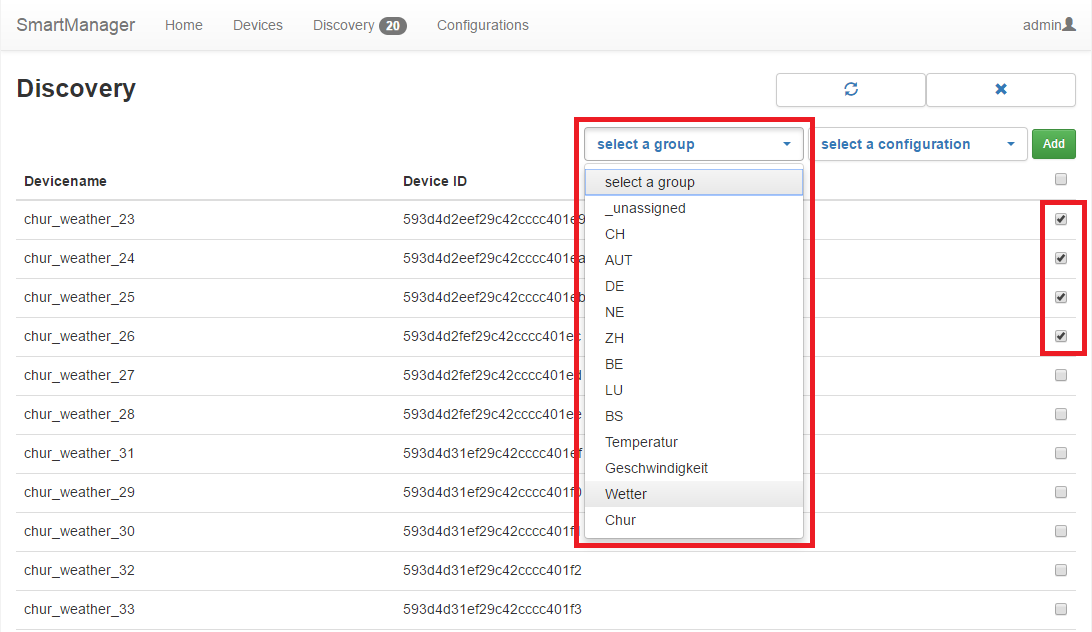
\includegraphics[scale=0.57]{../04_Realisierung/images/userinterface/discovery_addgroup.png}
\caption{Discovery Gruppenauswahl}
\end{figure}

Die selektierten Werte in den Drop-Down-Listen werden dem Server beim Hinzufügen des Devices übergeben.

\subsubsection{Refresh/Clear}
Mit dem Refresh Button wird die Seite neu geladen, damit frisch registrierte Devices angezeigt werden. Der Clear Button leert die Liste von Devices. Melden sich die Devices zu einem späteren Zeitpunkt nochmals, so tauchen sie in dieser Ansicht wieder auf.


\subsection{Devices und Groups}
\subsection{Configuration}




\section{Controllers}
\subsection{Rest}
\subsection{Web}


\begin{longtable}{ p{11cm} p{4cm} l}

\hline 
\multicolumn{1}{p{11cm}}{\textbf{URI}} & 
\multicolumn{1}{p{4cm}}{\textbf{Method}} &  \\ \hline 
\endfirsthead

\hline 
\multicolumn{1}{p{11cm}}{\textbf{URI}} & 
\multicolumn{1}{p{4cm}}{\textbf{Method}} &  \\ \hline 
\endhead

/	&	GET	 \\ \addlinespace
/login	&	GET	 \\ \addlinespace
/logout	&	GET	 \\ \addlinespace
/users	&	POST	 \\ \addlinespace
/users/add	&	POST	 \\ \addlinespace
/users/delete	&	POST	 \\ \addlinespace
/users/checkUser	&	POST	 \\ \addlinespace
/users/userAddFragment	&	GET	 \\ \addlinespace
/users/userDeleteFragment	&	GET	 \\ \addlinespace
/users/userEditFragment	&	GET	 \\ \addlinespace
/users/{id}/edit	&	POST	 \\ \addlinespace
/discovery	&	GET	 \\ \addlinespace
/discovery/clean	&	GET	 \\ \addlinespace
/configurations	&	GET	 \\ \addlinespace
/configurations/add	&	POST	 \\ \addlinespace
/configurations/createConfigurationFragment	&	GET	 \\ \addlinespace
/configurations/delete	&	POST	 \\ \addlinespace
/configurations/{id}/editConfigurationFragment	&	GET	 \\ \addlinespace
/devices	&	GET	 \\ \addlinespace
/devices/add	&	POST	 \\ \addlinespace
/devices/deleteAll	&	DELETE	 \\ \addlinespace
/devices/locations/dashboard	&	GET	 \\ \addlinespace
/devices/{id}	&	GET	 \\ \addlinespace
/devices/{id}/changeMembership	&	POST	 \\ \addlinespace
/devices/{id}/delete	&	DELETE	 \\ \addlinespace
/devices/{id}/memberships	&	GET	 \\ \addlinespace
/devices/{id}/removeFromGroups	&	POST	 \\ \addlinespace
/devices/{id}/locations/{mapType}	&	GET	 \\ \addlinespace
/devices/{id}/read/{objectId}	&	GET	 \\ \addlinespace
/devices/{id}/execute/{objectId}/{objectInstanceId}/{resourceId}	&	GET	 \\ \addlinespace
/devices/{id}/write/{objectId}/{objectInstanceId}/{resourceId}	&	POST	 \\ \addlinespace
/devices/{id}/read/{objectId}/{objectInstanceId}/{resourceId}	&	GET	 \\ \addlinespace
/groups/add	&	POST	 \\ \addlinespace
/groups/getAll	&	GET	 \\ \addlinespace
/groups/list	&	GET	 \\ \addlinespace
/groups/executeCommandToChildsFragment	&	GET	 \\ \addlinespace
/groups/writeCommandToChildsFragment	&	GET	 \\ \addlinespace
/groups/writeConfigToChildsFragment	&	GET	 \\ \addlinespace
/groups/{id}	&	GET	 \\ \addlinespace
/groups/{id}/add	&	POST	 \\ \addlinespace
/groups/{id}/changeMembers	&	POST	 \\ \addlinespace
/groups/{id}/changeMembership	&	POST	 \\ \addlinespace
/groups/{id}/delete	&	DELETE	 \\ \addlinespace
/groups/{id}/members	&	GET	 \\ \addlinespace
/groups/{id}/memberships	&	GET	 \\ \addlinespace
/groups/{id}/writeChildDevices/{objectId}/{objectInstanceId}/{resourceId}	&	GET	 \\ \addlinespace
/groups/{objectId}/executeToChildren	&	GET	 \\ \addlinespace
/groups/{objectId}/multiInstance	&	GET	 \\ \addlinespace
/groups/{objectId}/writeToChildren	&	GET	 \\ \addlinespace
/groups/{id}/executeChildDevices/{objectId}/{objectInstanceId}/{resourceId}	&	GET	 \\ \addlinespace
/groups/{id}/writeChildDevices/{objectId}/{objectInstanceId}/{resourceId}	&	GET	 \\ \addlinespace

\hline\caption{\textbf{Web API}}
\end{longtable}





\section{Services}




\newpage

\section{LwM2M-Server}
\subsection{Allgemein}
Damit sich die LwM2M-Clients bei dem Management-Tool melden können, wird ein LwM2M-Server benötigt. In diesem Projekt wurde der Leshan-Server in der Version 1.0.0 verwendet. Diese LwM2M Implementation beinhaltet eine Server- sowie eine Clientumsetzung des LwM2M-Protokolls. Entwickelt wird diese Library von dem Eclipse Project. Leshan baut auf der CoAP implementation Californium auf. Diese wurde von der ETH Zürich entwickelt und  gehört inzwischen auch zum Eclipse Project.

\subsection{Leshan Server}
\subsubsection{Adresse und Port}
Der LwM2M-Server wird mit der Klasse ''LwM2MManagementServer'' erstellt. Im Default Konstruktor setzt man dazu den gewünschten Port und Adresse.
Hier sieht man das Beispiel für den lokalen Start des Servers. Der Port 5683 ist dabei der Default Port von CoAP.
\begin{lstlisting}[language=java]
public LwM2MManagementServer() {
		this.address = "127.0.0.1";
		this.port = 5683;
}
\end{lstlisting}
\subsubsection{Object Models}
Jeder Leshanserver benötigt Object Model definitionen. Diese werden als XML im Projektordner abgelegt und danach als File-Object eingebunden.
Die Variable resource gibt dabei den Pfad zu den Models an:
\begin{lstlisting}[language=java]
private Resource resource = new ClassPathResource("ch/hsr/smartmanager/resources/models/");
\end{lstlisting}
Jedes Object Model, welches sich in diesem Pfad befindet wird von dem Server geladen und kann vom Server dargestellt werden. Benötigt man weitere Object Modelle, hinterlegt man diese in diesem Ordner und starten den Smartmanager neu. Schon hat man die neuste Definition beim Server hinterlegt.
\subsubsection{Create Methode}
Damit der Server bei jedem Start von Spring mitgestartet wird, wurde eine createServer-Methode erstellt und mit der Annotation @PostConstruct versehen. Für das erstellen des Servers wurde der LeshanServerBuilder verwendet. Dies ist eine einfache Möglichkeit einen Server zu erstellen und diesen danach zu starten.

Hier sieht man die Implementation der createServer-Methode. Als ersten Schritt fügt man eine Adresse und einen Port hinzu. Danach wird ein Encoder sowie ein Decoder. Nun können die oben erwähnten Object Models geladen und hinterlegt werden. Diese werden vom dem LwM2mModelProvider verwaltet.

Diese Angaben reichen bereits um einen Standardserver zu erstellen. Es wird noch ein RegistrationListener hinzugefügt, der weiter unten erklärt wird. Der Server wird nun einem TaskExecuter übergeben, um ihn zu starten.

\begin{lstlisting}[language=java]
@PostConstruct
public void createServer() {
	LeshanServerBuilder builder = new LeshanServerBuilder();

	builder.setLocalAddress(address, port);
		
	builder.setEncoder(new DefaultLwM2mNodeEncoder());
	LwM2mNodeDecoder decoder = new DefaultLwM2mNodeDecoder();
	builder.setDecoder(decoder);

	File file;
	try { file = resource.getFile(); } 
	catch (IOException e) { file = null; }

	models.addAll(ObjectLoader.load(file));
	LwM2mModelProvider modelProvider = new StaticModelProvider(models);
	builder.setObjectModelProvider(modelProvider);

	this.server = builder.build();
		
	server.getRegistrationService().addListener(
		registrationListenerImpl.getRegistrationListener()
	);
		
	serverTaskExecutor.doIt(this.server);
}
\end{lstlisting}
 
\subsection{RegistrationListener}
Der LeshanServer hat einen Registrierungsdienst, welche auf neue Anfragen hört. Um einen Zugriff auf diesen zu erhalten, muss man einen neuen RegistrationListener implementieren. Dieser erweitert danach den Standardlistener und gibt dadurch Zugriff auf die Registred-, Unregistred- und Update-Methoden. So kann das Gerät direkt nach der Registrierung im Management erfasst werden. 

Hier sieht man die einfache Umsetzung des in Smartmanager eingesetzten RegistrationListener. Einzige Funktion ist das hinzufügen oder anpassen der Registrierung. Unregistered wird nicht verwendet, da der User ein Device behalten kann, um weiter zugriff auf die Daten zu erhalten. 

\begin{lstlisting}[language=java]
@Service
public class RegistrationListenerImpl {

	@Autowired
	private DeviceService deviceService;

	public RegistrationListener getRegistrationListener() {

		return new RegistrationListener() {
			@Override
			public void registered(Registration registration) {
				updateOrAddDevice(registration);
			}

			@Override
			public void unregistered(Registration registration, Collection<Observation> observerColl) {}

			@Override
			public void updated(RegistrationUpdate registrationUpdate, Registration registration) {
				updateOrAddDevice(registration);
			}

		};
	}
}
\end{lstlisting}

\subsection{Server TaskExecutor}
Um den Server zu Starten, wird ein TaskExecutor von dem Spring Framework verwendet. Dazu wird ein Thread erzeugt und in diesem wird der Server durch server.start() gestartet. Der Thread wird danach dem TaskExecutor übergeben und gestartet.
\begin{lstlisting}[language=java]
public class ServerTaskExecutor {
	private class StartTask implements Runnable {

		private final LeshanServer server;

		public StartTask(LeshanServer server) {
			this.server = server;
		}
		public void run() {
			server.start();
		}
	}

	private TaskExecutor taskExecutor = new SimpleAsyncTaskExecutor();
	public void doIt(LeshanServer server) {
		taskExecutor.execute(new StartTask(server));
	}
}
\end{lstlisting}

\newpage

\section{Database}
\subsection{Allgemein}
Als Datenbank wurde eine MongoDB in der Version 3.4.3 verwendet. Zusätzlich wurden die Pakete mongo-java-driver (v3.4.2), spring-data-jpa (v3.4.2) spring-data-mongodb (v1.11.1) sowie spring-data-commons (v1.13.1) verwendet. Dadurch konnten wir uns sehr viel Codearbeit ersparen, da wir so schon vorgefertigte Repositories eingebunden haben.

Die Datenbank wurde bei der Implementierung lokal gehostet, könnte aber auch leicht auf eine Cloudumgebung ausgelagert werden. Die Datenbank beinhaltet vier Collections: Device, DeviceGroup, ManagementUser und Configuration. Zusätzlich zu jeder Collection gibt es ein Interface mit den angebotenen Repository-Methoden.
\subsection{Anbindung}
Für die Anbindung der Datenbank wurde das Spring Framework verwendet. In der der Datei ''smartmanager-servlet.xml'' wurden dazu folgendes Bean und der MongoDB Eintrag hinterlegt:
\begin{lstlisting}[language=xml]
<mongo:db-factory id="mongoDbFactory" client-uri="mongodb://localhost/smartmanager" />

<bean id="mongoTemplate" class="org.springframework.data.mongodb.core.MongoTemplate">
	<constructor-arg name="mongoDbFactory" ref="mongoDbFactory" />
</bean>
\end{lstlisting}
Dies reicht dem Spring Framework bereits aus, um die Datenbankverbindung herzustellen. Möchte man nun den Pfad der Datenbank auf einen Cloudservice wechseln, gibt man eifach eine andere Client-Uri an.

\subsection{Repositories}
Spring unterstützt bereits vorgefertigte Repositories. Um diese einzubinden, muss man in der ''smartmanager-servlet.xml'' einen ''mongo:repositories''-Eintrag hinterlegen. In diesem wird das Package, in welchem die Repository-Klassen und Interfaces liegen, hinterlegt.
\begin{lstlisting}[language=xml]
<mongo:repositories base-package="ch.hsr.smartmanager.data.repositories" />
\end{lstlisting}

\subsubsection{Library Methoden}
Pro Datanklasse, welche gespeichert werden soll, wird ein Interface erstellt. Dieses Interface extended das Interface MongoRepository. Dadurch erhält man viele Methoden, wie zum Beispiel findOne() oder save() und muss diese nicht selbst implementieren. Dieses Interface muss nach einem Schema benannt werden. Und zwar beginnt sie immer mit dem Datenklassenname und wird mit ''Repository'' erweitert. Hier sieht man ein Beispiel des DeviceRepository. Wichtig ist dabei die Annotation @Repository, damit Spring dieses Interface findet. 
\begin{lstlisting}[language=java]
@Repository
public interface DeviceRepository extends MongoRepository<Device, String>, DeviceRepositoryCustom {
	
	List<Device> findByAdded(boolean added);
	boolean existsByName(String name);
	Device findByName(String name);
}
\end{lstlisting}

Möchte man weitere Methoden zur Verfügung stellen, können diese im Interface erfasst werden. Dabei können viele Methoden ohne Implementierung erstellt werden. Dazu nimmt man die existierenden Methoden wie zum Beispiel ''find'' und hängt das gewünschte Feld als Namen an. Zum Beispiel ''findByName'' oder ''findbyLastUpdate'' generiert automatisch eine Methode, welche die Datenbank nach dem Datenklassenfeld ''Name'' oder ''LastUpdate'' durchsucht. So können schon sehr viele Methoden einfach und schnell angeboten werden. Ist das angegebene Feld nicht in der Datenklasse vorhanden, gibt Spring einen Fehler aus und startet nicht.

Es gibt bei den selbst erstellten Methoden aber noch Einschränkungen. Es können keine RemoveBy... Methoden erstellt werden. Für diese muss man immer eine Custom-Implementation erstellen.

\subsubsection{Custom Methoden}
Um eigene Methoden anzubieten, kann man eine Custom-Implementation erstellen. Für dies wird ein weiteres Interface und eine weitere Klasse benötigt. Hier ist die Namensgebung wieder entscheidend, da die Klassen sonst von Spring nicht gefunden werden.

Zuerst wird ein Interface mit <Datenklassennamen>RepositoryCustom als Namen erstellt. Hier ist wieder die Annotation @Repository notwendig. Dies ist ein Beispiel des DeviceRepositoryCustom-Interfaces. Alle benötigten Methoden werden hier erfasst.
\begin{lstlisting}[language=java]
@Repository
public interface DeviceRepositoryCustom {

	void removeDeviceByAddedIsFalse();
	void removeDeviceByName(String name);
}
\end{lstlisting}

Danach erstellt man eine Klasse mit dem Namen <Datenklassennamen>RepositoryImpl und implementiert die einzelnen Methoden. Dazu verwendet man die Klasse MongoTemplate, um die vorgefertigten Methoden, wie zum Beispiel Remove oder Save, einsetzen zu können. Durch die Query-Klasse kann man jede Abfrage abbilden und so nach spezielleren Kriterien filtern, anstelle von nur einzelnen Felder.

Hier sieht man ein Beispiel Query, welche alle Devices entfernt, bei denen Added False ist. 
\begin{lstlisting}[language=java]
public class DeviceRepositoryImpl implements DeviceRepositoryCustom {

	@Autowired
	private MongoTemplate mongoTemplate;

	@Override
	public void removeDeviceByAddedIsFalse() {
		Query query = new Query();
		query.addCriteria(Criteria.where("added").is(false));
		mongoTemplate.remove(query, Device.class);
	}
	...
}
\end{lstlisting}
\subsection{Collections}
Jede zu speichernde Datenklasse muss mit der Annotation @Document erstellt werden. Daduch weiss Spring, dass es sich hier um ein Document handelt, welches in eine Collection gehört. Spring erzeugt dadurch automatisch eine Collection mit dem Klassennamen.

Zusätzlich wird eine Id und ein leerer Default Konstruktor benötigt. Die Id benötigt auch eine @Id Annotation und sollte wenn möglich den Datentyp String oder ObjectId haben. Es gibt noch weitere Annotations, wie zum Beispiel @Indexed, aber es diese wurden bei diesem Projekt nicht verwendet. 
\begin{lstlisting}[language=java]
@Document
public class Device implements DeviceComponent {

	@Id
	private String id;

	private String name;
	private String regId;
	...
	
	public Device() {}
\end{lstlisting}

\subsection{Datenbanobjekt}
In der Datenbank wird jede Datenklasse als JSON-Objekt abgespeichert. Dieses beinhaltet alle Felder der Klasse, sowie eine generierte Id und eine Klassendefinition. Dadurch kann Spring das Objekt sehr einfach wieder zu einem Javaobject umwandeln und zur Verfügung stellen.

Hier sieht man ein Device, wie es auf der Datenbank gespeichert sein kann. Alle Datumsformate werden automatisch in ISODate umgewandelt und alle Ids werden von String in ObjectId umgewandelt. Alle anderen Typen sind nativ unterstützt und müssen nicht weiter umgewandelt werden.
\begin{lstlisting}[language=json]
{ 
	"_id" : ObjectId("593ab77b3f56e9309bbb4cf1"), 
	"_class" : "ch.hsr.smartmanager.data.Device", 
	"name" : "chur_weather_104", 
	"regId" : "tEBwKboGWD", 
	"endpoint" : "coap://127.0.0.1;42941", 
	"lastUpdate" : ISODate("2017-06-09T14:58:03.228Z"), 
	"latitude" : "44.0", 
	"longitude" : "-30.0", 
	"lastRegistrationUpdate" : ISODate("2017-06-09T15:38:34.117Z"),
	"objectLinks" : [ "/1/0", "/3/0", "/3303/0", "/6/0" ], 
	"added" : true, 
	"dataMap" : {  } 
}
\end{lstlisting}

\newpage

\subsection{Demo LwM2M-Client}
\subsection{Allgemein}
Wie auch der Server, ist der LwM2M-Client mit der Leshan Library implementiert. 
Raspberry Pi mit einem Arch Linux + Java Umgebung.
Temperatursensor und Lichtsensor.
Democlient von Leshan übernommen und angepasst.